\section{Experiment}
\label{sec_experiment}
In this Section, we firstly present the experimental setup, secondly we conduct intensive experiment to validate our observations. 

\vspace{-1ex}
\subsection{Experimental Setup}
\label{subsec_experiment_stup}
{\bf Hardware configuration.}
We conduct our experiments on a Terasic DE5a-Net board with an Altera Arria 10 GX FPGA and 8GB 2-bank DDR3 device memory. We design our kernels using Altera OpenCL SDK version 16.1. The FPGA board is connected to the host via a x8 PCI-e 3.0 interface.
	

{\bf Workloads. }We carry out our experiment with 11 OpenCL applications, as shown in in Table~\ref{t_dataset}. 
For example, eight applications are from Chai benchmark~\cite{chang2017collaborative}, which is highly optimized for GPUs.%one application is from Rodinia~\cite{rodinia_iiswc09}.

\begin{table}%[hbp]
    \centering
        \begin{scriptsize}
    \begin{tabular}{|c|c|c|c|c|c|}
        \hline
        Application & Source & AO & MPS & KKC & Datasets \\
        \hline
        BFS & \multirow{8}{*}{Chai~\cite{chang2017collaborative}} & Y & N & N & NY, NE, UT \\
        \cline{1-1} \cline{3-6}
        RSCD &  & Y & N & Y & 2000 iterations \\
        \cline{1-1} \cline{3-6}
        TQH &  & Y & N & N & Basket \\
        \cline{1-1} \cline{3-6}
        HSTI &  & Y & N & N & 256 bins \\
        \cline{1-1} \cline{3-6}
        BS &  & N & N & N & 4*4 \\
        \cline{1-1} \cline{3-6}
        SC &  & Y & Y & N & 50\% \\
        \cline{1-1} \cline{3-6}
        PAD &  & Y & Y & N & 1000*999 \\
        \cline{1-1} \cline{3-6}
        CEDD &  & N & N & Y & Peppa, Maradona, Paw \\
        \hline
        KM & Rodinia~\cite{rodinia_iiswc09} & N & N & N & 25600 points, 8 features \\
        \hline
        MM & \multirow{2}{*}{Intel demos} & N & N & N & A: 2048*1024, B: 1024*1024 \\
        \cline{1-1} \cline{3-6}
        MS &  & N & N & N & 640*800, 2000 iterations \\
        \hline
    \end{tabular}
        \end{scriptsize}
    \caption{Experimental datasets with OpenCL patterns}
    \vspace{-5.5ex}
    \label{t_dataset}
\end{table}

{\bf Comparison Methodology. }
Our evaluations mainly validate two hypotheses. First, different execution model leads to a significant performance difference (Subsection~\ref{subsec_evaluation}). Second, we can use three OpenCL patterns to determine the right OpenCL execution model (Subsection~\ref{subsection_connection}).  

\vspace{-1ex}
\subsection{Impact of Execution Model}
\label{subsec_evaluation}
In this subsection, we mainly validate that the right execution model leads to a significant performance speedup for the OpenCL application when mapping to FPGAs. In particular, we first try our best effort\footnote{Based on our more than five years' experience in programming FPGA with OpenCL, we are pretty sure that we have already found the near-optimal optimization combination for each execution model if available. } to explore the optimization combinations for each execution model of each OpenCL application, second quantitatively compare the highest performance speedup that each execution model can achieve. 


{\bf Exploring optimization combinations. }For each OpenCL application, we explore a broad range of optimization combinations for each execution model such that its performance potential has been harvested. Due to the space limitation, we take the application RSCD as an example. 
Figure~\ref{fig_optimization_combination} shows for each combination model, the performance speedup of each optimization combination over the baseline, which is optimized GPU code. X-axis is the optimization combination under all the four execution models. We can make two observations. 
First, different execution model yields an order of magnitude performance difference. In particular, the best optimization combination under ``NDRange+Channel" can achieve 43.4X, while 2.72X for the best combination under ``SWI". 
Second, the same optimization method can yield significantly different performance speedup under different execution models. For example, loop unrolling ``UL50" under ``SWI" can only achieve 1.26X performance speedup, while 43.4X under ``NDRange+Channel".  

 
%Second, SWI typically requires less memory traffic than NDRange. 
%Third, %NDRange can typically produce more parallelism than SWI.

\begin{figure*}[t]%\textwidth
	\centering
	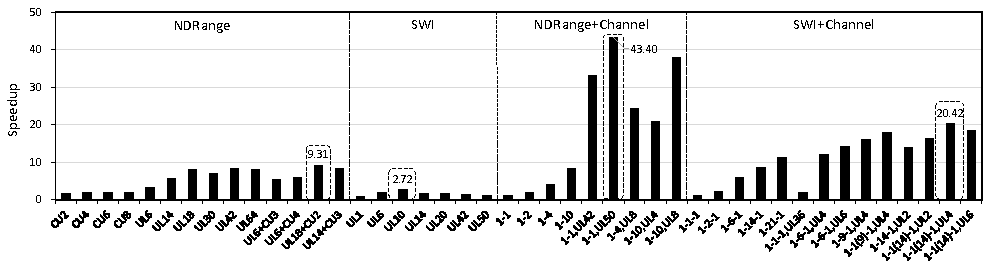
\includegraphics[width=6.05in]{rscd.pdf}
	\vspace{-3.2ex}
	\caption{Performance speedup of optimization combinations over baseline. ``CUx'' indicates x CUs, ``ULx'' indicates the loop whose unroll factor x. x-y(z)-w indicates XXX. }% We focus on the FPGA and main memory.
	\vspace{-3ex}
	\label{fig_optimization_combination}
\end{figure*} 



{\bf Speedup comparison of execution models. }
Table~\ref{t_optimization_combination} demonstrates for each execution model, the number of optimization combinations we have tried and maximum performance speedup over the baseline application which is directly imported from each source, e.g., Chai. 
We can make two observations. First, different execution model indeed results in significant performance speedup difference. Take HSTI as an example, the right execution model (SWI+Channel) can have 19.54X performance speedup over the baseline which is the optimized GPU code, while the inappropriate execution model (SWI) can only achieve 1.01X speedup. Second, different OpenCL application requires different execution model to achieve the best performance. For example, the best execution model for BFS is SWI+Channel, while NDRange is most suitable for MM. We conclude that it is critical to decide the right execution model when optimizing OpenCL application on FPGAs.  

%\begin{table}%[hbp]
%	\centering
%	\begin{scriptsize}
%		\begin{tabular}{|c|c|c|c|c|}
%			\hline
%			Application & NDRange & SWI & NDRange+Channel & SWI+Channel  \\
%			
%			
%			\hline
%			KM & 114.86 & 2.73 & 136.41 & 28.96 \\
%			\hline
%			BFS & 1.6 & 2.77 & 1.19 & 2.94 \\ 
%			\hline
%			RSCD & 9.31 & 2.72 & 43.4 & 20.42 \\
%			\hline
%			TQH & 1 & 1.28 & & 2.98 \\
%			\hline
%			HSTI & 2.67 & 1.06 & 9.49 & 19.54 \\
%			\hline
%			BS & 3.01 & 10.77 & 3.34 & 44.06 \\
%			\hline
%			SC & 1.52 & 4.51 &  & 17.13 \\
%			\hline
%			PAD & 1 & 1.6 &  & 4.8 \\
%			\hline
%			CEDD & 2.95 & 0.02 & 2.72 & 0.03 \\
%			\hline
%			MM & 837.12 & 0.73 & & 0.72 \\
%			\hline
%			Mandelbrot & 34.72 & 2.48 & & 3.17  \\
%			
%			\hline
%		\end{tabular}
%	\end{scriptsize}
%	\caption{Optimization combinations: number and speedup }
%	\label{t_optimization_combination}
%\end{table}


\begin{table}%[hbp]
	\centering
	\begin{scriptsize}
		\begin{tabular}{|c|c|c|c|c|c|c|c|c|}
			\hline
		    \multirow{2}{*}{Application} & \multicolumn{4}{c|}{Number of combinations} & \multicolumn{4}{c|}{Maximum speedup} \\
         \cline{2-9}
			
			 %& NDRange & SWI & NDRange+Channel & SWI+Channel & NDRange & SWI & NDRange+Channel & SWI+Channel \\
			& NDR & SWI & NDR+C & SWI+C & NDR & SWI & NDR+C & SWI+C \\
			
			\hline
			KM & 30 & 14 & 12 & 17 & 147.67 & 8.76 & 136.41 & 28.96 \\
			\hline
			BFS & 17 & 1 & 1 & 4 
			& 1.85 & 2.95 & 1.22 & 2.96 \\ 
			\hline
			RSCD & 22 & 10 & 24 & 39 & 9.31 & 2.72 & 43.4 & 20.42 \\
			\hline
			TQH & 1 & 15 & & 20 & 1 & 1.28 & & 2.98 \\
			\hline
			HSTI & 9 & 36 & 9 & 28 & 2.67 & 1.06 & 9.49 & 19.71 \\
			\hline
			BS & 20 & 17 & 18 & 8 & 3.01 & 10.77 & 3.34 & 44.06 \\
			\hline
			SC & 15 & 34 & & 9 & 1.52 & 4.51 &  & 17.13 \\
			\hline
			PAD & 11 & 10 && 14 & 1.15 & 1.6 &  & 4.8 \\
			\hline
			CEDD & 55 & 9 & 25 & 2 & 2.95 & 0.01 & 2.72 & 0.02 \\
			\hline
			MM & 25 & 3 && 1 & 837.12 & 0.73 & & 0.72 \\
			\hline
			MS & 7 & 6 && 7 & 34.72 & 0.02 & & 3.17  \\
			
			\hline
		\end{tabular}
	\end{scriptsize}
	\caption{Space exploration of optimization combinations }
	\label{t_optimization_combination}
	\vspace{-5ex}
\end{table}





 

%Hypotheses to validate:Evaluation of 

\vspace{-1ex}
\subsection{Prediction of Right Execution Model}
\label{subsection_connection}
In this subsection, we mainly validate that for each OpenCL application, the prediction of execution model matches the empirical result. Essentially, we can predict the right execution model, which can produce best performance, based on three OpenCL patterns (Section~\ref{sec_bridge_gap}). Table~\ref{t_prediction_execution_model} shows the predicted execution model, as well as the real execution model which can achieve the best performance in our real experiment. 
We can observe that the prediction of execution model almost matches the real experimental result.    
%Second, .



\begin{table}%[hbp]
	\centering
	\begin{scriptsize}
		\begin{tabular}{|c|c|c|c|c|c|}
			\hline
			Application & AO & MPS & KKC & Real & Prediction\\
			
			% the 3 pattern's name is too long
			
			\hline
			BFS & Y & N & N & SWI+Channel & SWI+Channel  \\
			\hline
			RSCD & Y & N & Y & NDRange+Channel & SWI+Channel \\
			\hline
			TQH & Y & N & N & SWI+Channel & SWI+Channel \\
			\hline
			HSTI & Y & N & N & SWI+Channel & SWI+Channel \\
			\hline
			BS & N & N & N & SWI+Channel & NDRange \\
			\hline
			SC & Y & Y & N & SWI+Channel & SWI+Channel \\
			\hline
			PAD & Y & Y & N & SWI+Channel & SWI+Channel \\
			\hline
			CEDD & N & N & Y & NDRange & NDRange+Channel \\
			\hline
			KM & N & N & N & NDRange & NDRange \\
			\hline
			MM & N & N & N & NDRange & NDRange \\
			\hline
			MS & N & N & N & NDRange & NDRange \\
			\hline
		\end{tabular}
	\end{scriptsize}
	\caption{Prediction of execution model}
	\label{t_prediction_execution_model}
	\vspace{-5ex}	
\end{table}



